%-----------------Präambel-----------------%
\documentclass[a0,portrait]{a0poster}
\usepackage{multicol}
\usepackage[utf8]{inputenc}
\usepackage[T1]{fontenc}
\usepackage{ae}
\usepackage{lmodern}
\usepackage{helvet}
\renewcommand{\familydefault}{\sfdefault}
\newcommand{\changefont}[3]{\fontfamily{#1} \fontseries{#2} \fontshape{#3} \selectfont}
\usepackage[ngerman]{babel}
\usepackage{color}
\definecolor{darkgreen}{rgb}{0,0.5,0}
\definecolor{darkblue}{rgb}{0,0,0.5}
\definecolor{bluesky}{rgb}{0.63,0.80,1.0}
\usepackage{amsmath}
\usepackage{amssymb}
\usepackage{fancybox}
\usepackage{graphicx}
\usepackage{blindtext}
%-----------------Makros-----------------%
\renewcommand\baselinestretch{1.35}
\parskip=0.5\baselineskip
\parindent0mm %Einrücktiefe der ersten Zeile eines Absatzes
\topmargin-28pt
\marginparwidth0mm

%Ränder rechts/links

\oddsidemargin-13pt
\evensidemargin-13pt
\textwidth785mm
%\textheight1140mm

\newcommand{\spaltenbreite}{15}
\newcommand{\bildbreite}{15cm}

\newcommand*\widefbox[1]{\noindent\frame{\hspace{1ex}\parbox{\dimexpr\textwidth\relax}{\vspace{0.5\baselineskip}#1\vspace{0.5\baselineskip}}\hspace{1ex}}}

\setlength{\fboxrule}{1.25mm} 		%Definiert die Linienstärke für nachfolgende fbox- und framebox-Befehle
\setlength{\fboxsep}{5mm} 			%Abstand zwischen Rahmen und Text bei den /fbox und /framebox Befehlen.
\setlength{\columnsep}{15mm}     	%Spaltenabstand
\setlength{\columnseprule}{0pt}  	%Balken zwischen Spalten {0pt}->keine Balken

\unitlength1cm


% Literaturverzeichnis:
\usepackage[autostyle=true,german=quotes]{csquotes}
\usepackage[
backend=biber,
style=iso-numeric,
autolang=other,
bibencoding=UTF8,
maxnames=3,
hyperref
]{biblatex}

\DefineBibliographyStrings{ngerman}{andothers={et\ al\adddot}}
{\def\section*#1{}\addbibresource{Referenzen.bib}}


\apptocmd{\UrlBreaks}{\do\f\do\m}{}{}
\setcounter{biburllcpenalty}{9000}% Kleinbuchstaben
\setcounter{biburlucpenalty}{9000}% Großbuchstaben

%-----------------Beginning-----------------%
\begin{document}

\begin{picture}(0,0)
\put(66.5, -6){
\includegraphics[height=60mm]{Bilder/fhl_logo.eps}}
\put(0.0, -3.5){
\includegraphics[height=33mm]{Bilder/cardioscan_logoclaim_RGB_pos.png}}
\end{picture}
\vspace{6cm}
\begin{center}
	\vspace*{0.00001\textheight}
	{\huge \textbf{Evaluierung von Methoden
			zur Bestimmung der ventilatorischen
			Schwellen in der Spiroergometrie}\\}%[0.03\textheight]
	\vspace*{0.025\textheight}
	
\end{center}

%\cornersize*{20mm}
\linethickness{0.5mm}
\setlength{\fboxrule}{1.0mm}


%%%%%%%%%%%%%%%%%%%%%%%%%%%%%%%%%%%%%%%%%%%%%%%%%%%%%%%%%%%%%%%%%%%%%%% 
% neuer Kasten
%\Ovalbox
\widefbox
{
	\parbox{\textwidth}{
		\begin{multicols}{3}
			\begin{center} \textbf{\Large Einleitung} \end{center}
Die Spiroergometrie (aus lat. \textsl{spirare}: atmen, griech. \textsl{ergo}: Arbeit) ist eine oft genutzte technische Anwendung der Sportmedizin zur Bestimmung von individuellen Trainingsbereichen, bei der respiratorische Daten während inkrementierter körperlicher Belastung erfasst und anschließend analysiert werden. Der Hamburger Medizintechnik-Hersteller cardioscan GmbH hat 2017 ein Spiroergometer entwickelt, welches in Verbindung mit einer Software für dieses Verfahren noch nicht getestet wurde. Die Software verwendet momentan einen Algorithmus, der recht sensitiv für Fehler ist und deshalb durch einen neuen ersetzt werden muss. Hierfür eignen sich Methoden zur Bestimmung der Ventilatorischen Schwellen VT1 und VT2, die von der AG Spiroergometrie empfohlen werden~\cite{Westhoff.2012}.\\
Es wurden im Rahmen dieser Arbeit insgesamt vier Methoden ausgewählt, die in Folge an eine Spiroergometrie mit dem neuen Gerät des Unternehmens bestimmt werden sollten. Zu überprüfen war, ob das Gerät generell für diese Anwendung nutzbar ist, welche der vier Methoden zum Erreichen der Firmenziele optimal ist und ob die Methoden genauere Ergebnisse liefern können, als der ursprüngliche Algorithmus.





			\begin{center} \textbf{\Large Grundlagen} \end{center}

Das ventilatorische Schwellenkonzept basiert auf der physiologischen Reaktion des Körpers auf die zunehmende Belastung bei einer Spiroergometrie. Da der Muskelgehalt des körpereigenen Energiestoffs ATP zur Muskelkontraktion nur für eine kurze Zeit ausreicht, muss dieser für andauernde Arbeit durch Glykolyse oxidativ resynthetisiert werden \cite{Kroidl.2015}. Reicht ab einer bestimmten Belastung die Sauerstoffaufnahme (\.{V}O\textsubscript{2}) nicht mehr aus, fehlen dem Körper gewisse Enzyme, sodass in den Muskeln Laktat akkumuliert und es allmählich zur metabolischen Azidose (Übersäuerung) kommt. Der Körper versucht, dies durch Puffer-Reaktionen zu kompensieren, wodurch überschüssiges Kohlenstoffdioxid (CO\textsubscript{2}) anfällt, welches respiratorisch messbar abgeatmet wird.\\
Bestimmte Atemparameter können grafisch verglichen werden, um die ventilatorische Reaktion auf metabolische Prozesse zu detektieren. Die sogenannten ventilatorischen Schwellen stellen die Stoffwechselübergänge dar, anhand derer mit verschiedenen Modellen Trainingsbereiche bestimmbar sind. Die VT1 kann mittels der V-Slope-Methode oder anhand des Sauerstoff-Äquivalents EQO\textsubscript{2} grafisch identifiziert werden. Das Kohlenstoffdioxid-Äquivalent EQCO\textsubscript{2} oder der Vergleich der Ventilation (\.{V}E) mit der Kohlenstoffdioxidabgabe (\.{V}CO\textsubscript{2}) eignen sich zur Bestimmung der VT2.\\

\begin{picture}(\spaltenbreite,6)
\put(0.5,2){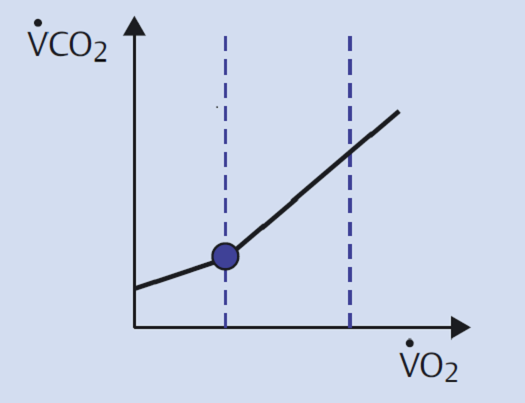
\includegraphics[width=50mm]{Bilder/vslope.png}}
\put(0.4,1){\parbox{720pt}{{\bf \small Abb. 1:} \small V-Slope}}
\put(6.7,2){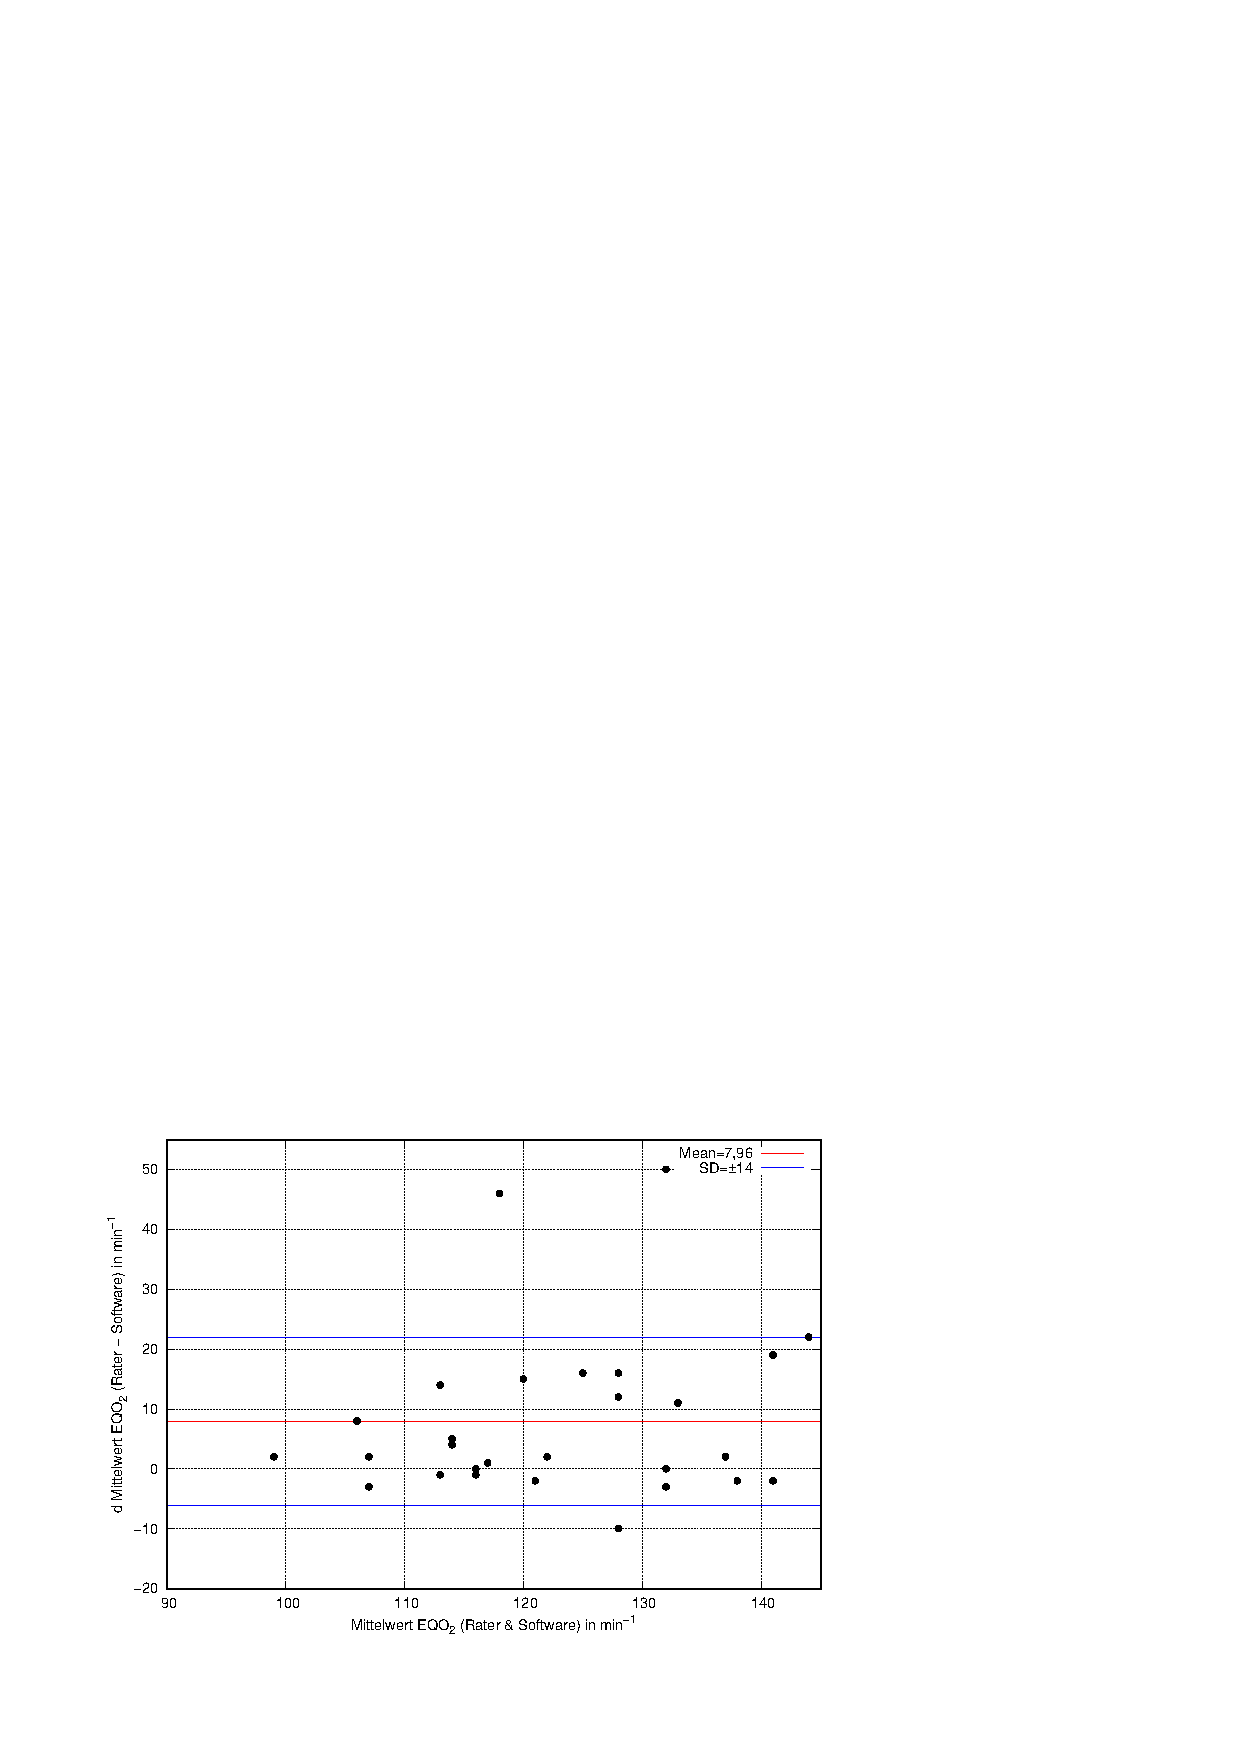
\includegraphics[width=50mm]{Bilder/eqo2.png}}
\put(6.9,1){\parbox{720pt}{{\bf \small Abb. 2:} \small EQO\textsubscript{2}}}
\put(12.9,2){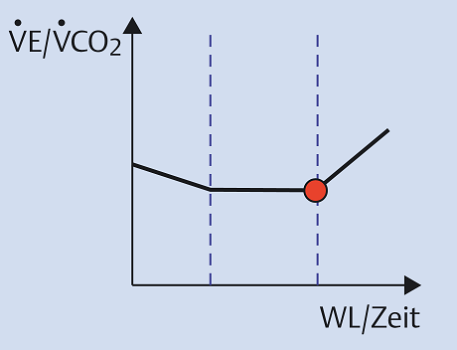
\includegraphics[width=50mm]{Bilder/eqco2.png}}
\put(12.9,1){\parbox{720pt}{{\bf \small Abb. 3:} \small EQCO\textsubscript{2}}}
\put(19.2,2){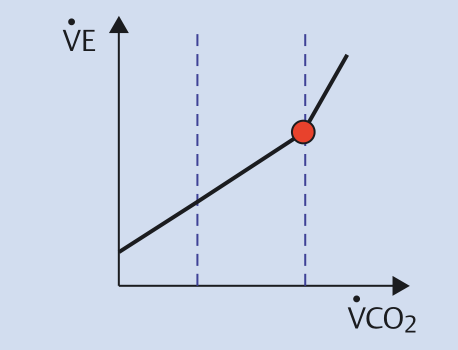
\includegraphics[width=50mm]{Bilder/field4.png}}
\put(18.9,1.1){\parbox{720pt}{{\bf \small Abb. 4:} \small \.{V}E/\.{V}CO\textsubscript{2}}}
\end{picture}

		\end{multicols}
	}
}

% neuer Kasten
\vspace*{0.01\textheight}
%\Ovalbox
\widefbox
{
	\parbox{\textwidth}{
		\begin{multicols}{3}
			\begin{center} \textbf{\Large Methode} \end{center}

In einem firmeninternen Projekt wurden mit 28 unterschiedlichen Probanden nach einem gleichen festgelegten Prozedere spiroergometrische Tests auf einem Fahrradergometer durchgeführt, bei der die Herzfrequenz zusätzlich über einen Pulsgurt erfasst wurde. Die Sensor-Rohdaten des Spiroergometers, die Herzfrequenz sowie die Leistungswerte des Ergometers wurden durch ein MATLAB-Programm weiterverarbeitet und grafisch in Form von "`6-Felder-Grafiken"' visualisiert. In diesen sind die Plots für alle vier Methoden enthalten. Die Grafiken wurden subjektiv von zwei Ratern und mathematisch durch einen Algorithmus analysiert. Anschließend wurden die Ergebnisse der unterschiedlichen Methoden statistisch miteinander verglichen und Differenzen bzw. Abweichungen bei den identifizierten Schwellen untersucht. Die Ergebnisse wurden außerdem mit den Erkenntnissen HUNT 3 Studie aus dem Jahre 2014 verglichen, um zu evaluieren, ob die individuell gemessenen Werte realistisch waren.

			\vfill
			\columnbreak
			\textbf{\Large Resultate}
\vspace*{1.6em}\\
Bei den Testmessungen traten keinerlei Gerätefehler oder Störungen auf, sodass für alle 28 Probanden Ergebnisse in Form von Graphen erstellt werden konnten. Abb. 5 zeigt ein Beispiel einer 6-Felder-Grafik, in der die respiratorischen Parameter in verschiedenen Farben aufgetragen sind. Zum Ablesen der ventilatorischen Schwellen ist die entsprechend gemessene Herzfrequenz in Form einer rosafarbenen Linie in die Plots integriert.

\begin{center}
\begin{picture}(\spaltenbreite,16)
\put(-2.5,3){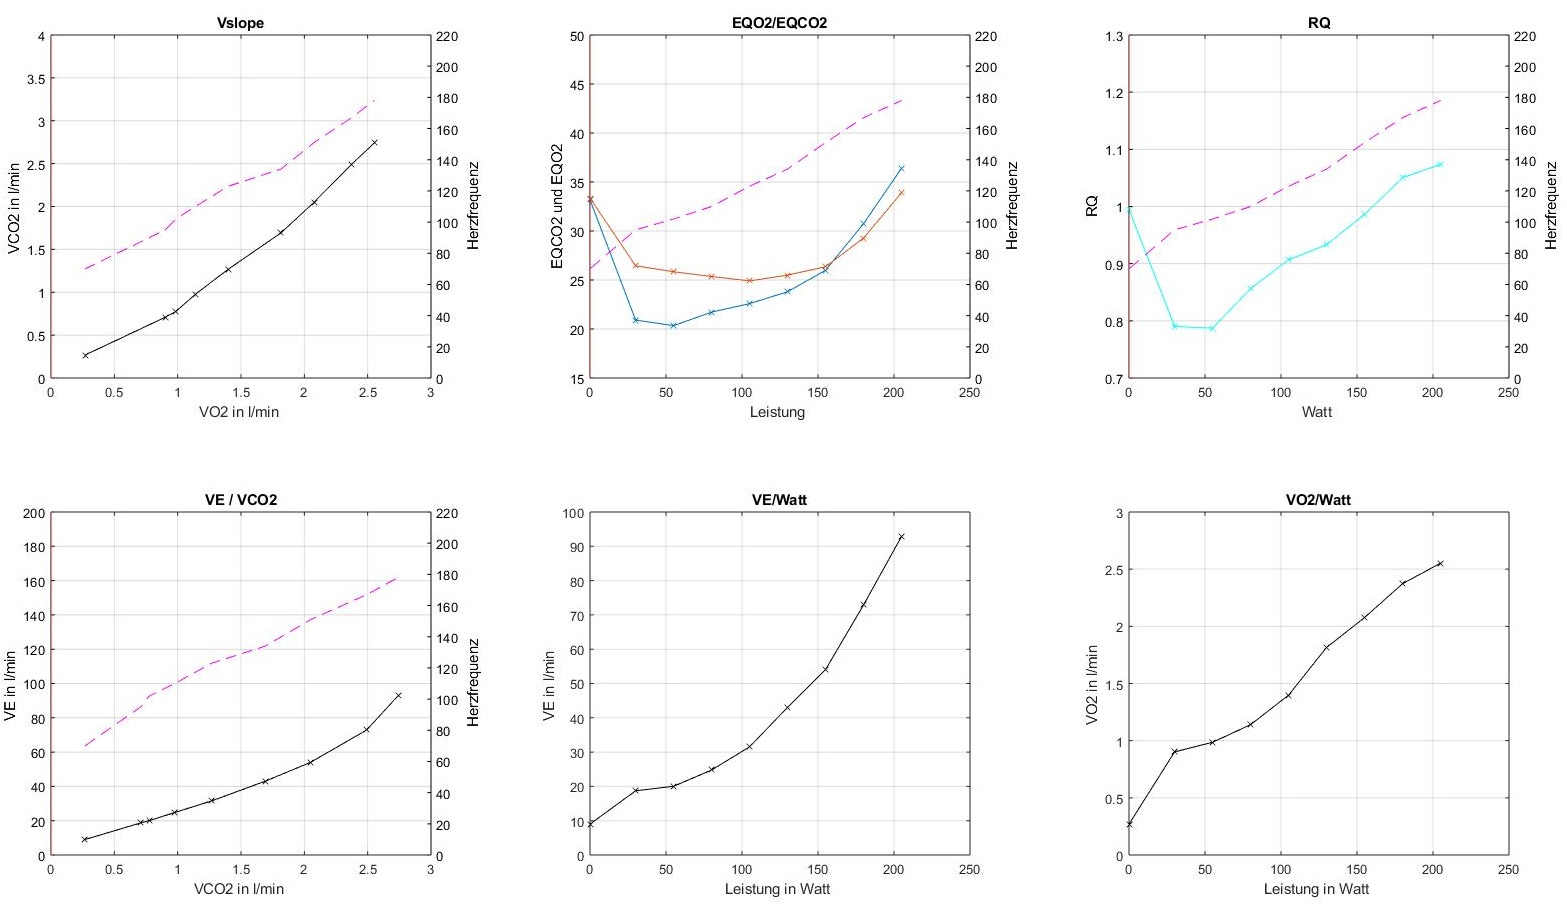
\includegraphics[width=200mm]{Bilder/plot_6w.jpg}}
\put(1.3,1.5){\parbox{720pt}{{\bf \small Abb. 5:} \small Beispiel einer 6-Felder-Grafik}}
\end{picture}
\end{center}


			\begin{center}
\begin{picture}(\spaltenbreite,20)
\put(-4,10){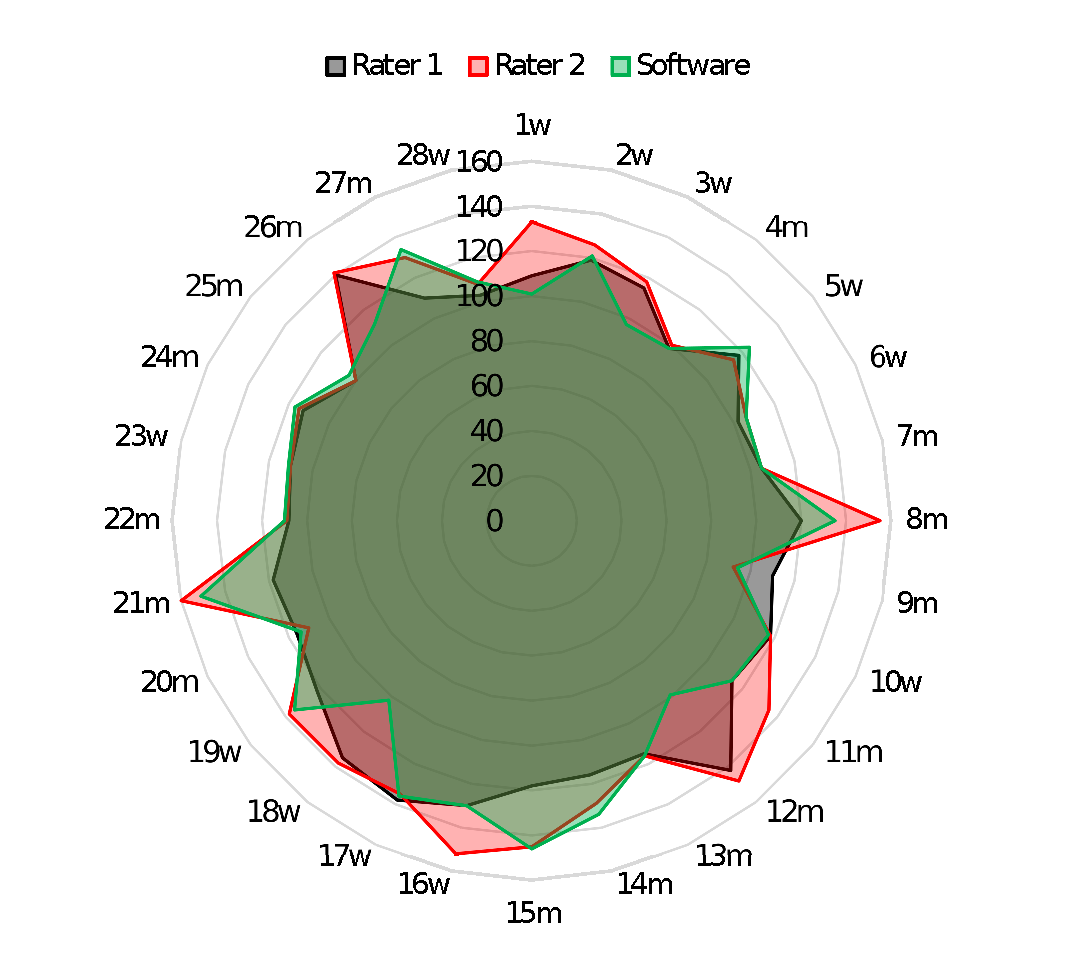
\includegraphics[width=110mm]{Bilder/v-slope_net.eps}}
\put(-0.8,9){\parbox{720pt}{{\bf \small a)} \small für V-Slope}}
\put(8,10){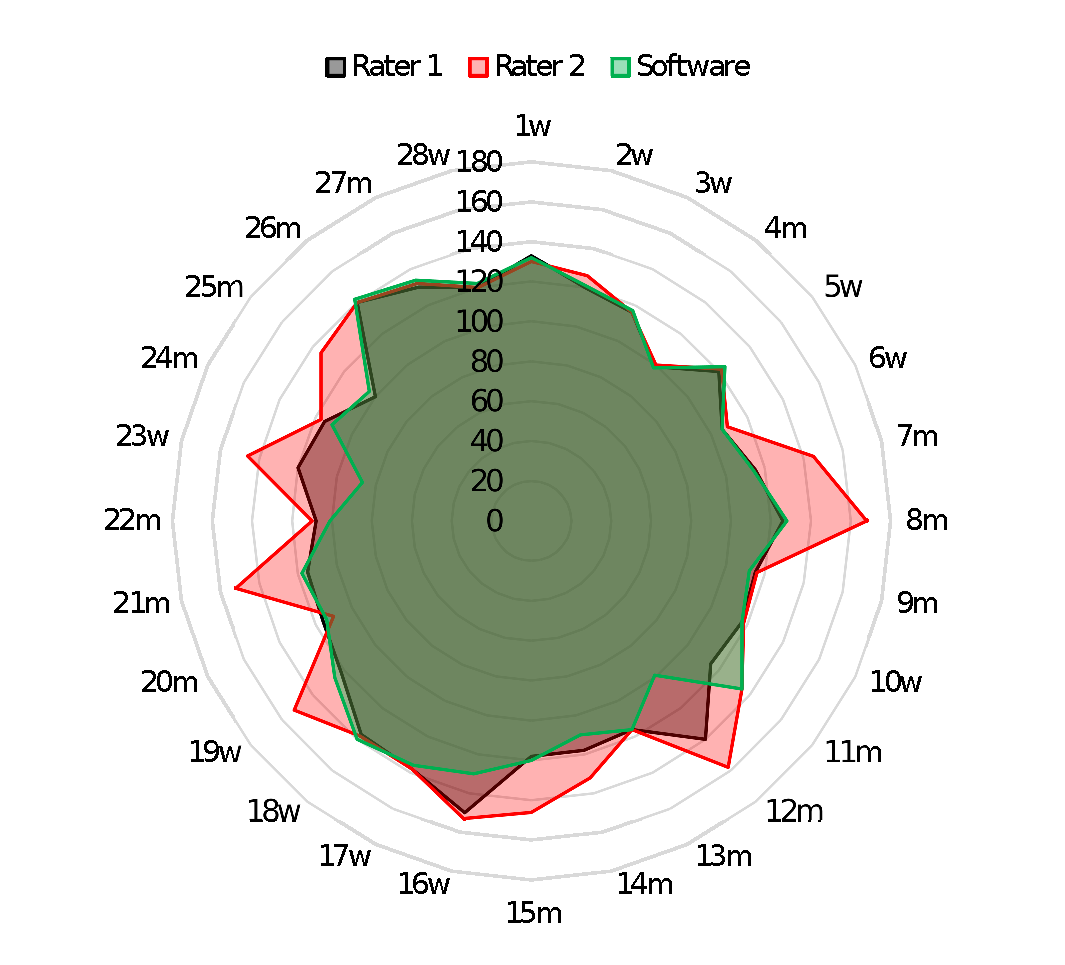
\includegraphics[width=110mm]{Bilder/eqo2_net.eps}}
\put(11.3,9){\parbox{720pt}{{\bf \small b)} \small für EQO\textsubscript{2}}}
\put(-4,-2){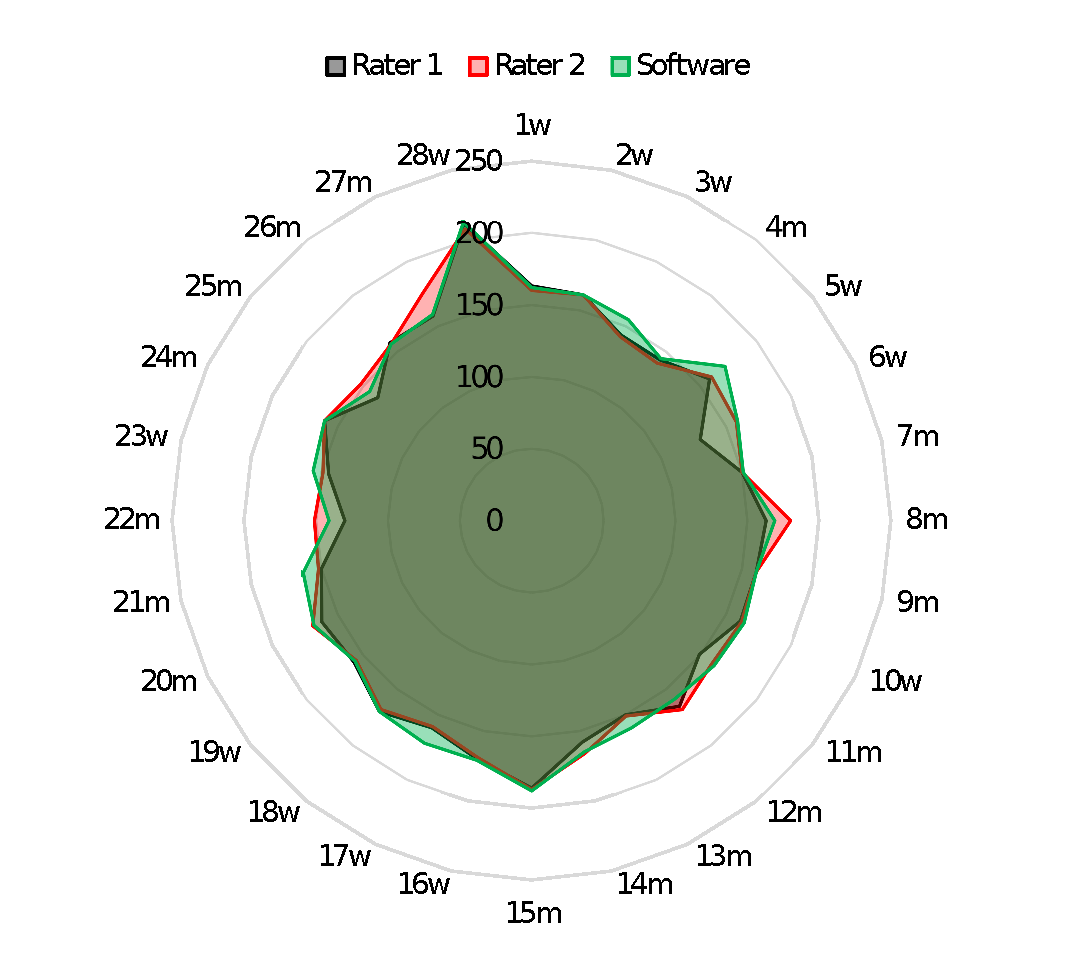
\includegraphics[width=110mm]{Bilder/eqco2_net.eps}}
\put(-0.7,-3){\parbox{720pt}{{\bf \small c)} \small für EQCO\textsubscript{2}}}
\put(8,-2){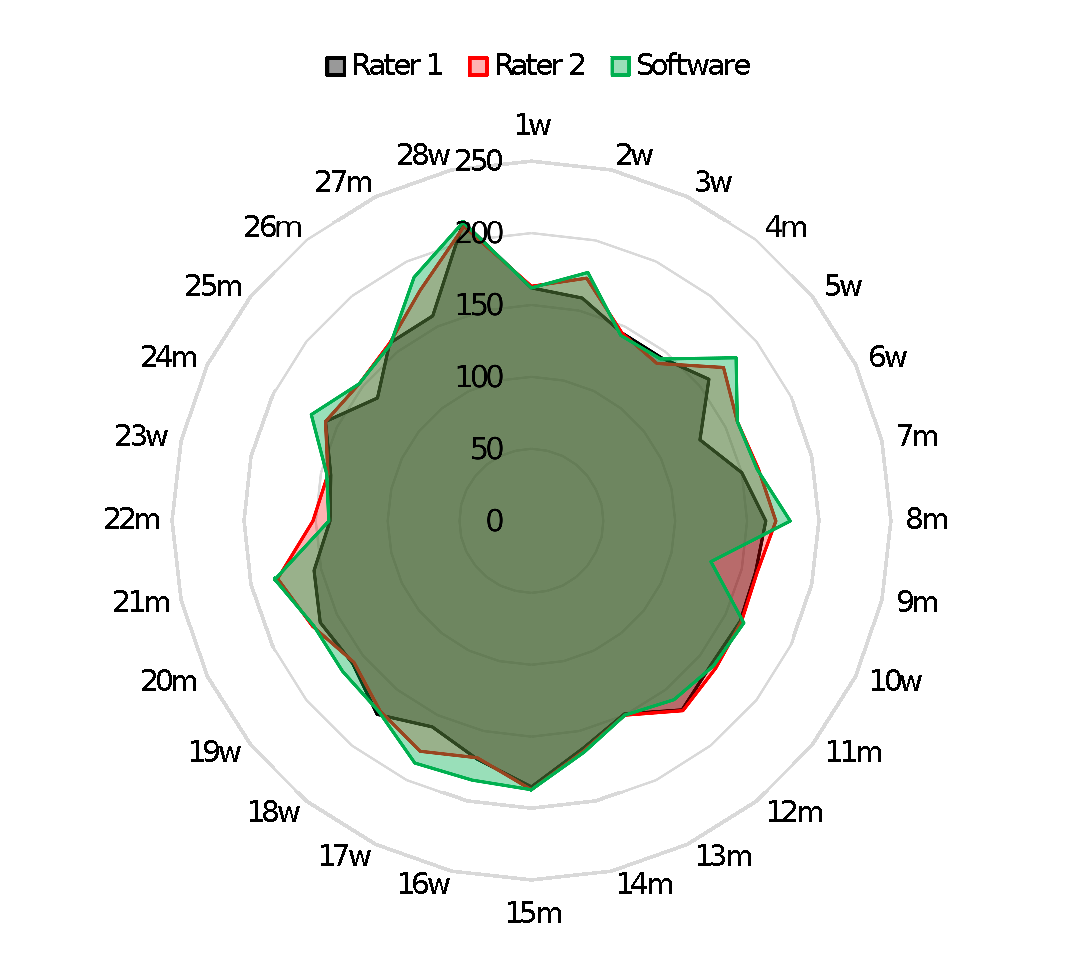
\includegraphics[width=110mm]{Bilder/vevco2_net.eps}}
\put(10.8,-3){\parbox{720pt}{{\bf \small d)} \small für \.{V}E/\.{V}CO\textsubscript{2}}}
\put(-0.85,-5){\parbox{720pt}{{\bf \small Abb. 3:} \small Verteilung der Ergebnisse für die Schwellen}}
\end{picture}
\end{center}
\vspace*{6.3cm}
Abb. 3 zeigt die unterschiedlichen Ergebnisse der Schwellenbestimmung der Rater und Software für die Probanden anhand der vier Methoden in Form von Netzdiagrammen.
		\end{multicols}
	}
}

\vspace*{0.01\textheight}
%\Ovalbox
\widefbox
{
	\parbox{\textwidth}{
		\begin{multicols}{3}
			\begin{center}
	\begin{picture}(\spaltenbreite,21)
	\put(-4,13){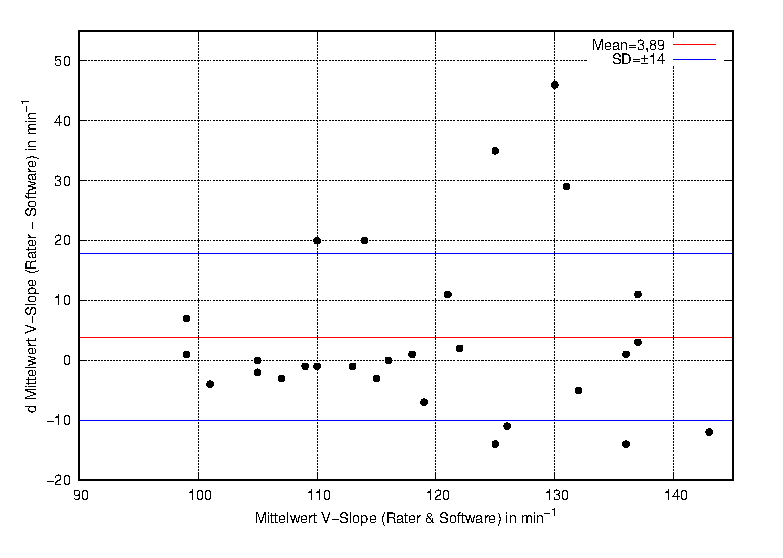
\includegraphics[width=110mm]{Bilder/vslope.eps}}
	\put(-0.8,12){\parbox{720pt}{{\bf \small a)} \small für V-Slope}}
	\put(8,13){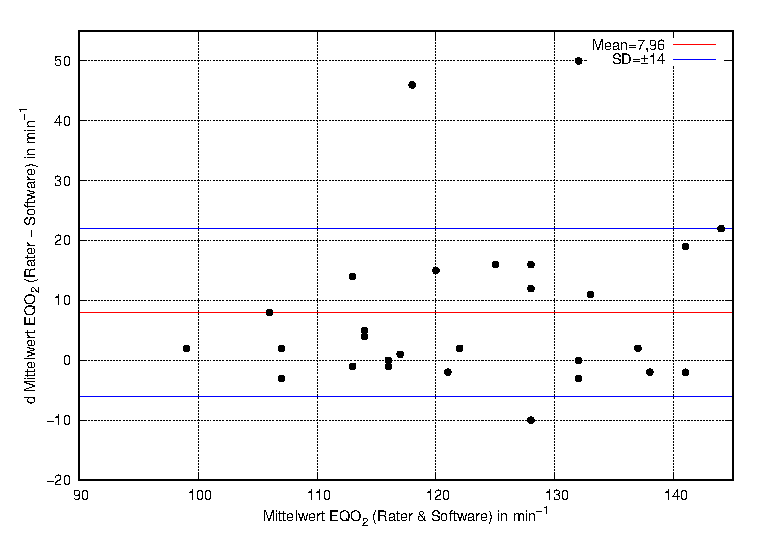
\includegraphics[width=110mm]{Bilder/eqo2.eps}}
	\put(11.5,12){\parbox{720pt}{{\bf \small b)} \small für EQO\textsubscript{2}}}
	\put(-4,3){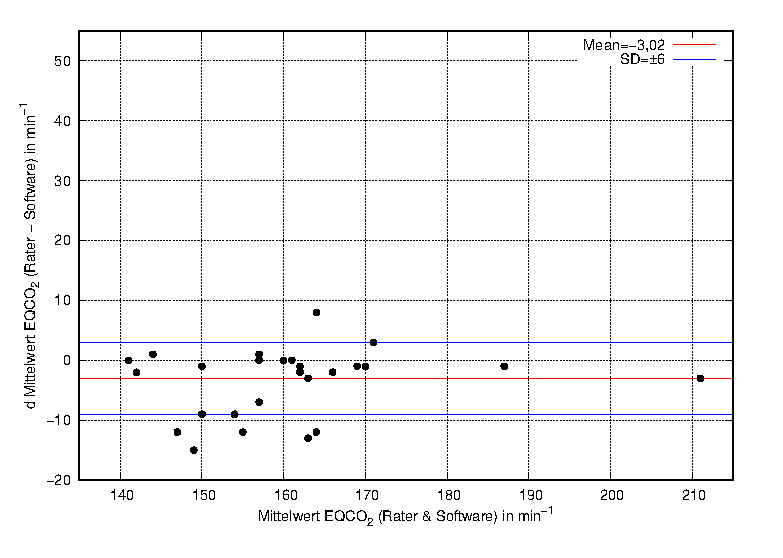
\includegraphics[width=110mm]{Bilder/eqco2.eps}}
	\put(-0.7,2){\parbox{720pt}{{\bf \small c)} \small für EQCO\textsubscript{2}}}
	\put(8,3){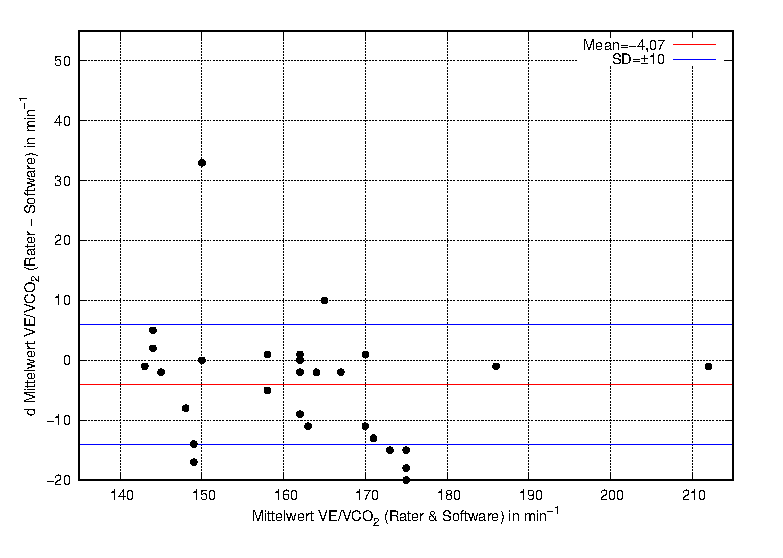
\includegraphics[width=110mm]{Bilder/vevco2.eps}}
	\put(11,2){\parbox{720pt}{{\bf \small d)} \small für \.{V}E/\.{V}CO\textsubscript{2}}}
	\put(-2.6,0.6){\parbox{720pt}{{\bf \small Abb. 4:} \small Streuung der Ergebnisse um die mittlere Abweichung}}
	\end{picture}
\end{center}
\vspace{1em}
Die Abb. 4 stellt zu diesen Ergebnissen die methodenspezifische Streuung der Schwellenbestimmungen um die mittlere Abweichung zzgl. der entsprechenden Standardabweichung (SD) dar.
\vspace{1em}


			\vfill
			\columnbreak
			\textbf{\Large Diskussion}\\

Abb. 6 zeigt, dass die Ergebnisse für die beiden VT1-Methoden häufig sehr stark streuen und für die VT2 wesentlich einheitlicher waren. In Abb. 7 ist zu erkennen, dass die EQCO\textsubscript{2}-Methode die insgesamt geringsten Differenzen zwischen den Ratern und der Software aufweist und dementsprechend am eindeutigsten ist. Der Korrelationskoeffizient für diese Methode beträgt $r = 0,912$. Zudem ist diese Methode genauer und zuverlässiger als die veraltete Methode und wurde darum in die Software implementiert.\\
Über die Hälfte der erhobenen Messwerte sind vergleichbar mit den Referenzdaten der HUNT 3 Studie~\cite{Loe.2014}, obwohl diese auf Laufbandergometern durchgeführt wurden. Den Erkenntnissen des Projektes folgend, wird angenommen, dass das Gerät des Unternehmens für die Spiroergometrie generell genutzt werden kann. Außerdem können mit der durch die EQCO\textsubscript{2}-Methode erhobenen VT2 nach einem Modell von Wilfried Kindermann Trainingszonen gemäß der Ziele des Unternehmens definiert werden~\cite{Kindermann.2004}.\\
Künftige Verbesserungen am Algorithmus, z.B. im Hinblick auf ein besseres Mittelungs-Verfahren für die Mittelwerte einer Belastungsstufe, könnten die Ergebnisse noch weiter optimieren.
		%	\vfill
		%	\columnbreak
			\nocite{*}
\printbibliography{}
		\end{multicols}
	}
}

\vspace*{0.01\textheight}
\begin{picture}(0,0)
\put(0,-0.9){\line(78,0){79.4}}
\put(0,-1.9){\textsf{\textbf{$\blacksquare${} Bachelorand: Julian-Marvin Lütten, Betreuer: Prof. Dr. Dipl.-Ing. Ullrich Wenkebach, Studiengang: Biomedizintechnik, 2018}}}
\end{picture}
\end{document}